% Created 2021-10-08 Fri 13:24
% Intended LaTeX compiler: pdflatex
\documentclass{article}
\usepackage[utf8]{inputenc}
\usepackage[T1]{fontenc}
\usepackage{graphicx}
\usepackage{grffile}
\usepackage{longtable}
\usepackage{wrapfig}
\usepackage{rotating}
\usepackage[normalem]{ulem}
\usepackage{amsmath}
\usepackage{textcomp}
\usepackage{amssymb}
\usepackage{capt-of}
\usepackage{hyperref}

\usepackage[a4paper,left=0.5in,right=0.5in,top=0.5in,bottom=1in]{geometry}
\usepackage{float}
\usepackage{enumerate}
\DeclareUnicodeCharacter{2212}{-}
\setcounter{secnumdepth}{0}
\author{Tzong Lin Chua}
\date{\today}
\title{EE4C10 Analog Circuit Design Fundamentals\\\medskip
\large Homework Assignment IV }
\hypersetup{
 pdfauthor={Tzong Lin Chua},
 pdftitle={EE4C10 Analog Circuit Design Fundamentals},
 pdfkeywords={},
 pdfsubject={},
 pdfcreator={Emacs 27.1 (Org mode 9.5)}, 
 pdflang={English}}
\begin{document}

\maketitle
\tableofcontents


\section{Simulation Files}
\label{sec:org7ffe627}
Each question with simulation files will have their respective subfolder.

Running the simulation files should be able to directly plot the graphs used (configured in the *.plt file).
The folders for each question are arranged as follows after extracting:

\begin{center}
\begin{tabular}{lll}
\hline
spice &  & \\
 & q3 & \\
 &  & a\\
 &  & b\\
 &  & c\\
 &  & d\\
 & q4 & \\
 &  & a\\
 &  & b\\
 &  & c\\
\hline
\end{tabular}
\end{center}
\section{Problem 1}
\label{sec:org2fb1c6b}
\begin{enumerate}[(a)]
\item DC gain, \(|\frac{V_{out}}{V_{in}}|\)

KCL at drain node,
\begin{equation*}
\begin{aligned}
\frac{V_{out}}{R_{D}} &= (g_{m} + g_{mb})v_{s} \\
\frac{V_{out}}{v_{s}} &= (g_{m} + g_{mb})R_{D} \\
\end{aligned}
\end{equation*}

KCL at source node,
\begin{equation*}
\begin{aligned}
\frac{V_{in} - V_{S}}{R_{S}} &= (g_{m} + g_{mb})v_{s} \\
\frac{V_{in}}{v_{s}} &= R_{S}(g_{m} + g_{mb}) + 1 \\
\end{aligned}
\end{equation*}

DC gain,
\begin{equation*}
\begin{aligned}
|\frac{V_{out}}{V_{in}}| &= \frac{(g_{m} + g_{mb})R_{D}}{(g_{m} + g_{mb})R_{S} + 1} \\
\end{aligned}
\end{equation*}

\item Pole of output node, \(\omega_{p,out}\)

\begin{equation*}
\begin{aligned}
R_{out} &= R_{D} \\
C_{out} &= C_{DB} + C_{GD} \\
\\
\omega_{p,out} &= \frac{1}{R_{D}(C_{DB} + C_{GD})} \\
\end{aligned}
\end{equation*}

\item Input impedance,

\begin{equation*}
\begin{aligned}
Z_{IN} &= \frac{1}{g_{m} + g_{mb} + s(C_{GS} + C_{SB})} \\
\end{aligned}
\end{equation*}

\item Source capacitance, \(C_{S}\), and input pole, \(\omega_{p, in}\),

\begin{equation*}
\begin{aligned}
C_{S} &= C_{GS} + C_{SB} \\
\\
\omega_{p, in} &= \frac{g_{m} + g_{mb} + R_{S}^{-1}}{C_{S}} \\
&= \frac{g_{m} + g_{mb} + R_{S}^{-1}}{C_{GS} + C_{SB}} \\
\end{aligned}
\end{equation*}
\end{enumerate}

\section{Problem 2}
\label{sec:org6c3ba6c}
\begin{enumerate}[(a)]
\item Transfer function, \(\frac{V_{out}(s)}{V_{in}(s)}\),

DC gain,
\begin{equation*}
\begin{aligned}
|\frac{V_{out}(S)}{V_{in}(s)}| &= 1 \\
\end{aligned}
\end{equation*}

Poles at gate and source nodes,
\begin{equation*}
\begin{aligned}
\omega_{p,G} &= \frac{1}{R_{S}(C_{GB} + G_{GD})} \\
\\
\omega_{p,D} &= \frac{g_{m}}{C_{SB}} \\
\end{aligned}
\end{equation*}

Transfer function,
\begin{equation*}
\begin{aligned}
\frac{V_{out}(S)}{V_{in}(s)} &= \frac{1}{1 + sR_{S}(C_{GB} + G_{GD})}\frac{1}{1 + s\frac{C_{SB}}{g_{m}}} \\
&= \frac{1}{(1 + sR_{S}(C_{GB} + G_{GD}))(1 + \frac{sC_{SB}}{g_{m}})} \\
\end{aligned}
\end{equation*}

\item Poles at gate and source nodes,
\begin{equation*}
\begin{aligned}
\omega_{p,G} &= \frac{1}{R_{S}(C_{GB} + G_{GD})} \\
\\
\omega_{p,D} &= \frac{g_{m}}{C_{SB}} \\
\end{aligned}
\end{equation*}

\item Input impedance,
\begin{equation*}
\begin{aligned}
Z_{in} &= \frac{1}{s(C_{GB} + C_{GD})} \\
\end{aligned}
\end{equation*}
\end{enumerate}
\section{Problem 3}
\label{sec:orgdf846e0}
\begin{enumerate}[(a)]
\item Testbench,
\begin{figure}[H]
\centering
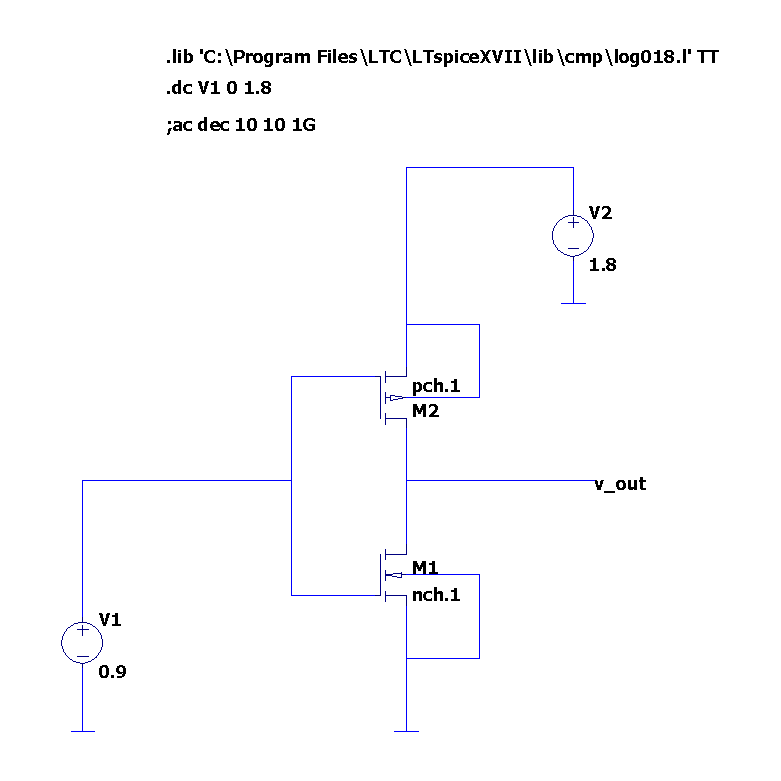
\includegraphics[height=300px]{img/q3/inverter.pdf}
\caption{\label{fig:inv-q3}Inverter testbench}
\end{figure}

DC transfer curve,
\begin{figure}[H]
\centering
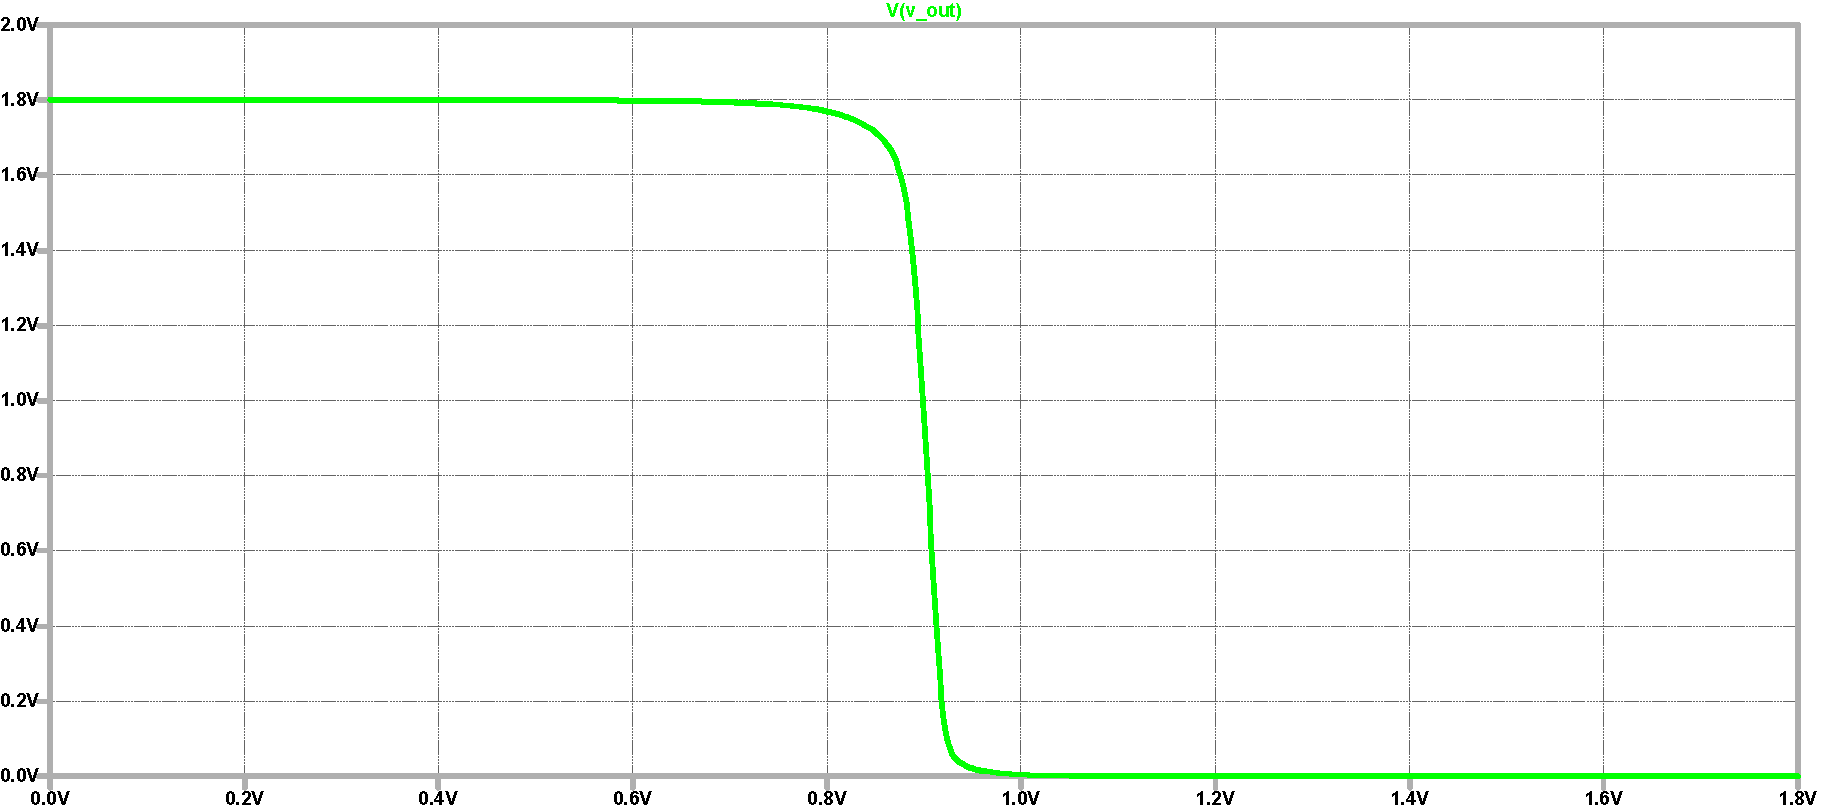
\includegraphics[width=.9\linewidth]{img/q3/vout-vin-dc.pdf}
\caption{\label{fig:vout-vin-dc-q3}Inverter DC response}
\end{figure}

\item Transient response,

\begin{figure}[H]
\centering
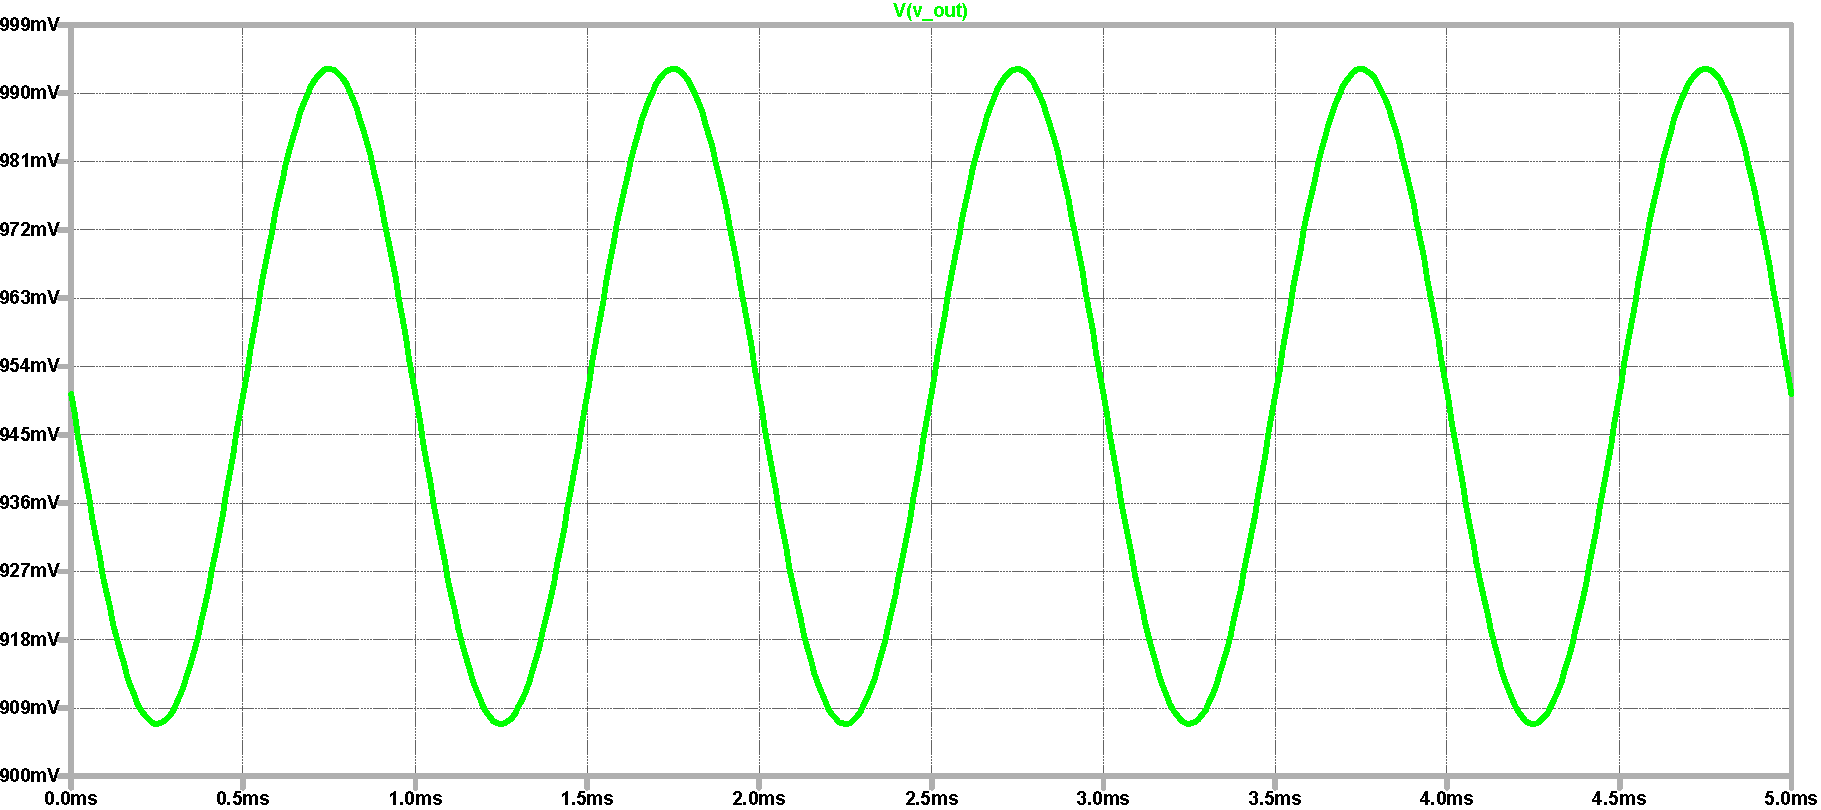
\includegraphics[width=.9\linewidth]{img/q3/transient.pdf}
\caption{\label{fig:trans-q3}Inverter transient response}
\end{figure}
\item AC responce

\begin{figure}[H]
\centering
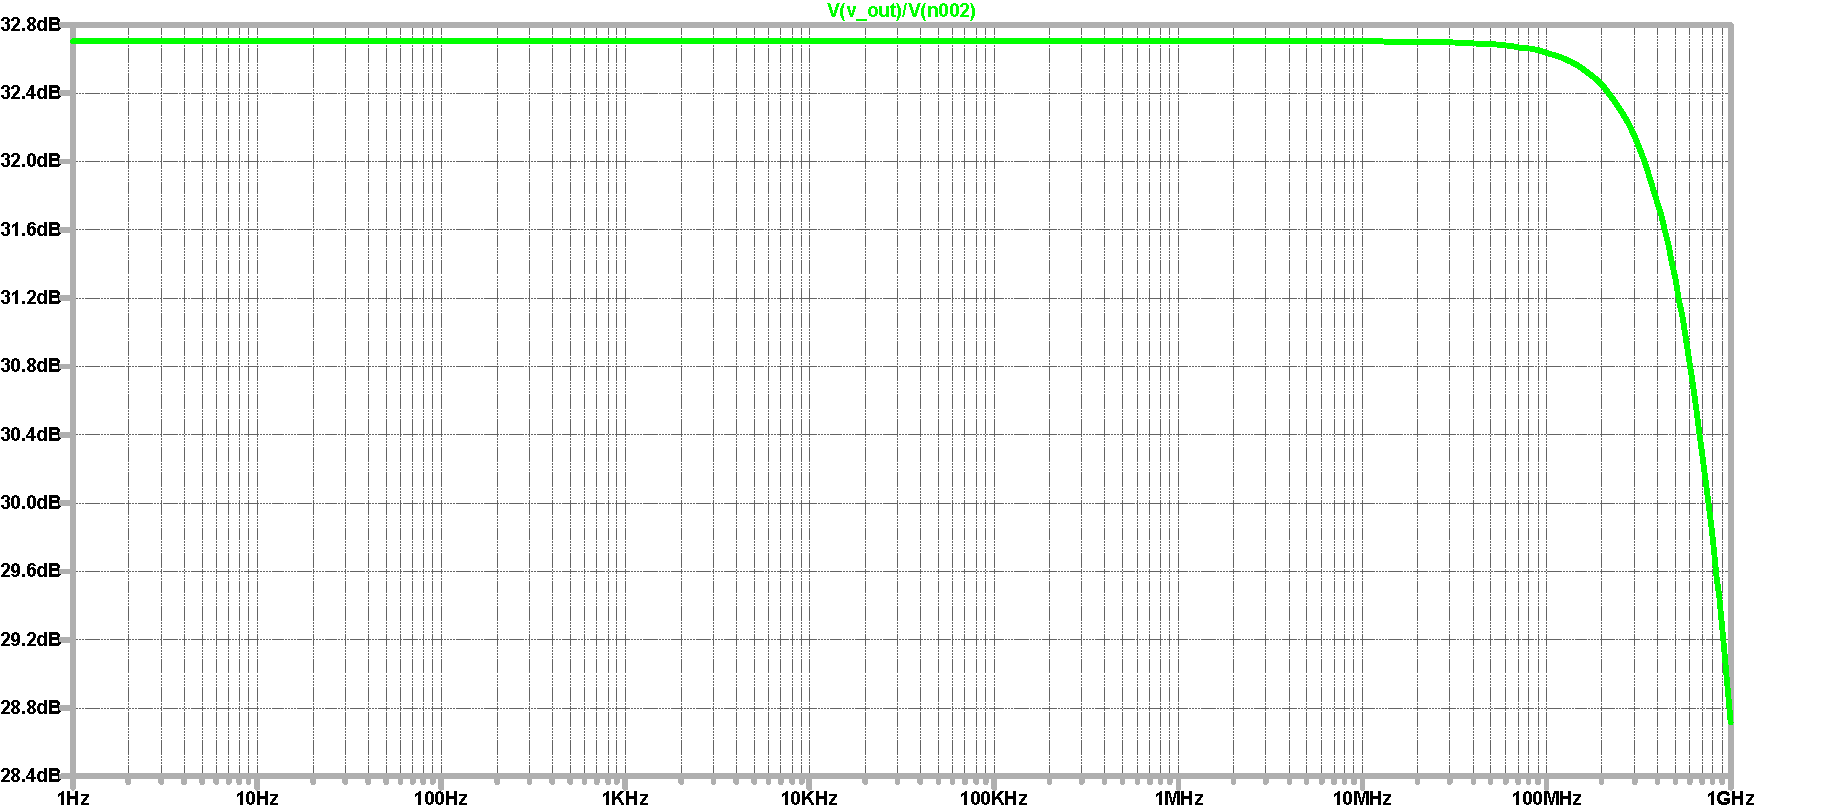
\includegraphics[width=.9\linewidth]{img/q3/gain-c.pdf}
\caption{\label{fig:gain-c-q3}Inverter AC gain}
\end{figure}

\begin{equation*}
\begin{aligned}
|\frac{V_{out}}{V_{in}}| &= 32.7dB \\
&= 43.2 \\
\omega_{p} &= 2\pi{}f_{-3dB} \\
&= 5.136 \times 10^{9} rad s^{-1} \\
\end{aligned}
\end{equation*}

\item AC Response

\begin{figure}[H]
\centering
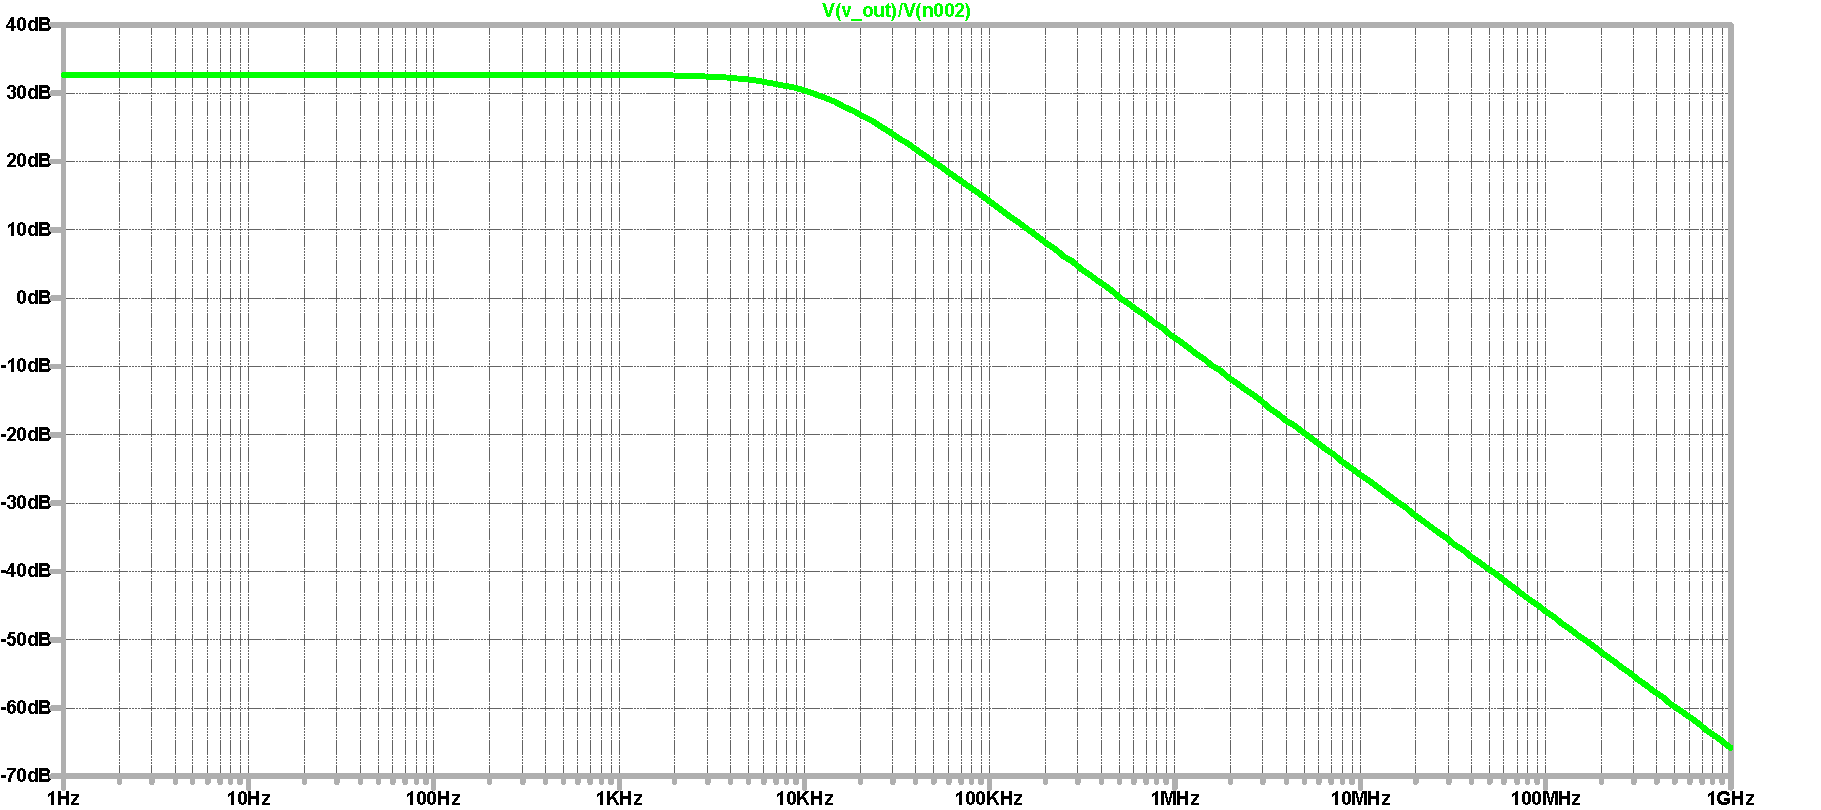
\includegraphics[width=.9\linewidth]{img/q3/gain-d.pdf}
\caption{\label{fig:gain-d-q3}Inverter AC gain with output capacitor}
\end{figure}

\begin{equation*}
\begin{aligned}
|\frac{V_{out}}{V_{in}}| &= 32.7 dB \\
&= 43.2 \\
\omega_{p} &= 2\pi{}f_{-3dB} \\
&= 7.42 \times 10^{4} rad s^{-1} \\
\end{aligned}
\end{equation*}

\item The pole at output node.

Since the added capacitance is much larger than capacitance of the transistors.
\begin{equation*}
\begin{aligned}
RC &\approx \frac{1}{2\pi{}f_{d}} \\
\\
R_{out} &= 134.75 k\Omega \\
\end{aligned}
\end{equation*}
\end{enumerate}

\section{Problem 4}
\label{sec:orgef146bd}
\begin{enumerate}[(a)]
\item Testbench
\begin{figure}[H]
\centering
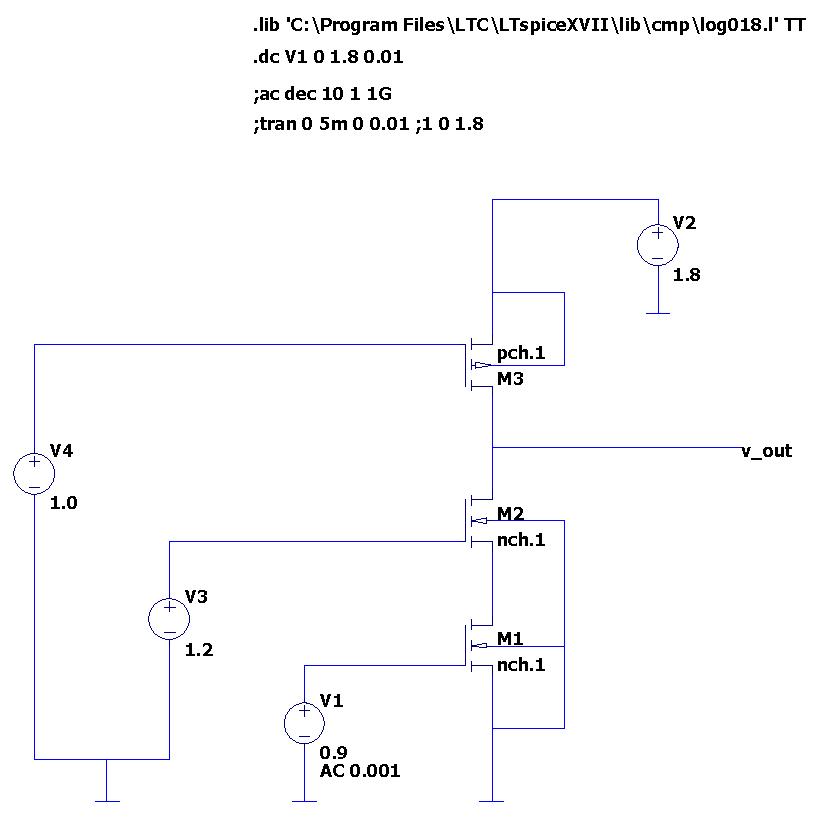
\includegraphics[height=300px]{img/q4/testbench.pdf}
\caption{\label{fig:testbench-q4}Testbench}
\end{figure}

DC transfer curve,
\begin{figure}[H]
\centering
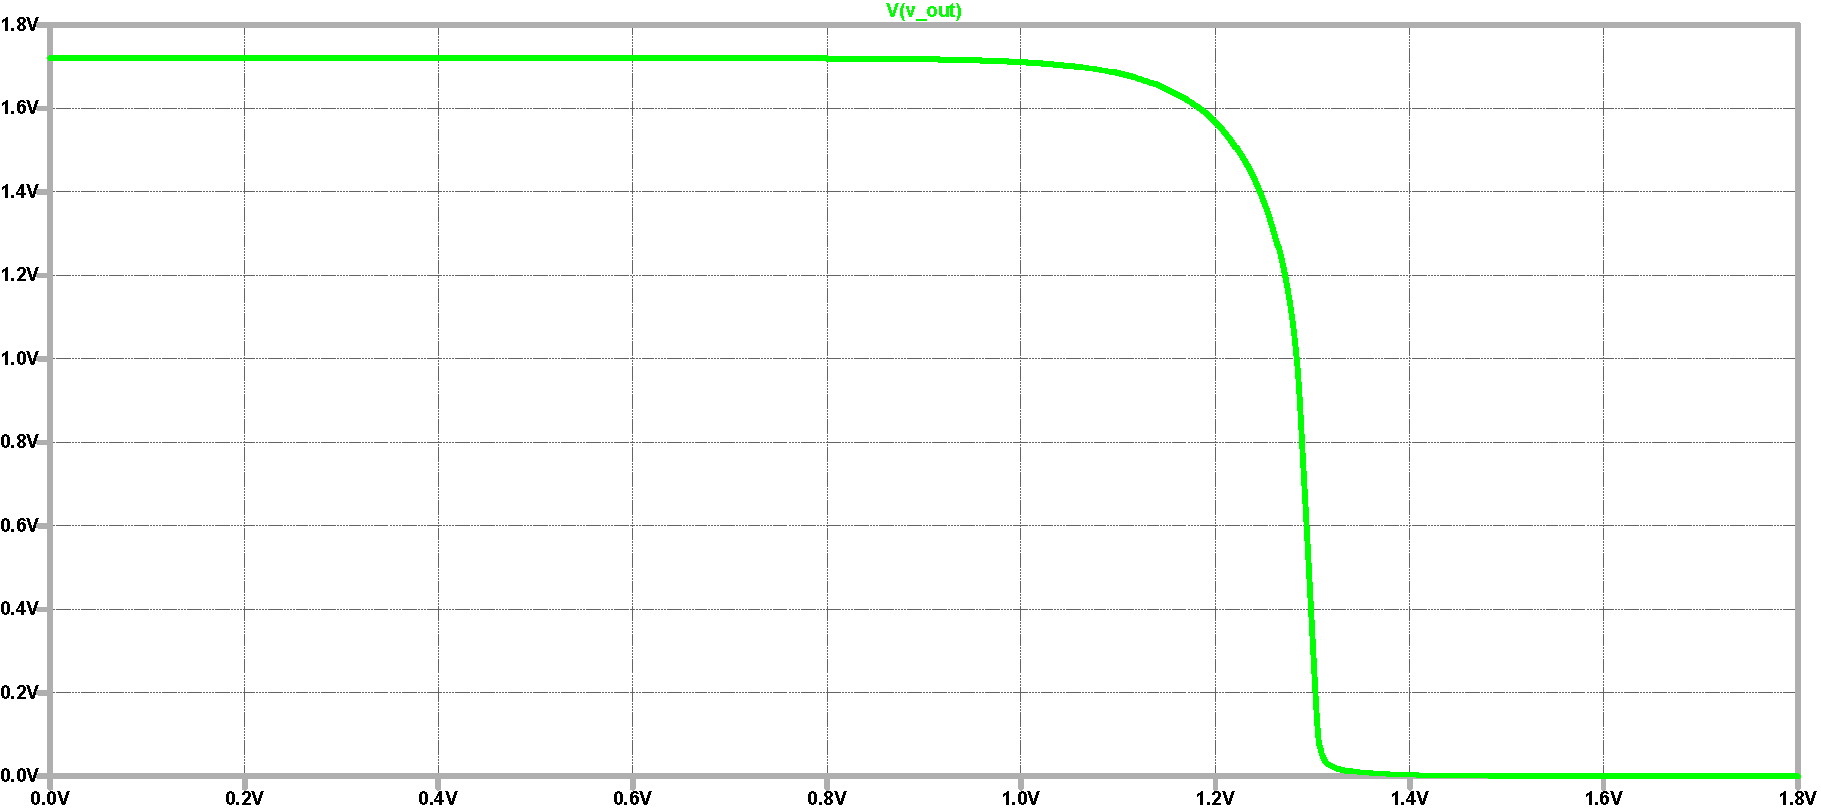
\includegraphics[width=.9\linewidth]{img/q4/vout-vin-dc.pdf}
\caption{\label{fig:vout-vin-dc-q3}DC response}
\end{figure}

\item Transient response,

\begin{figure}[H]
\centering
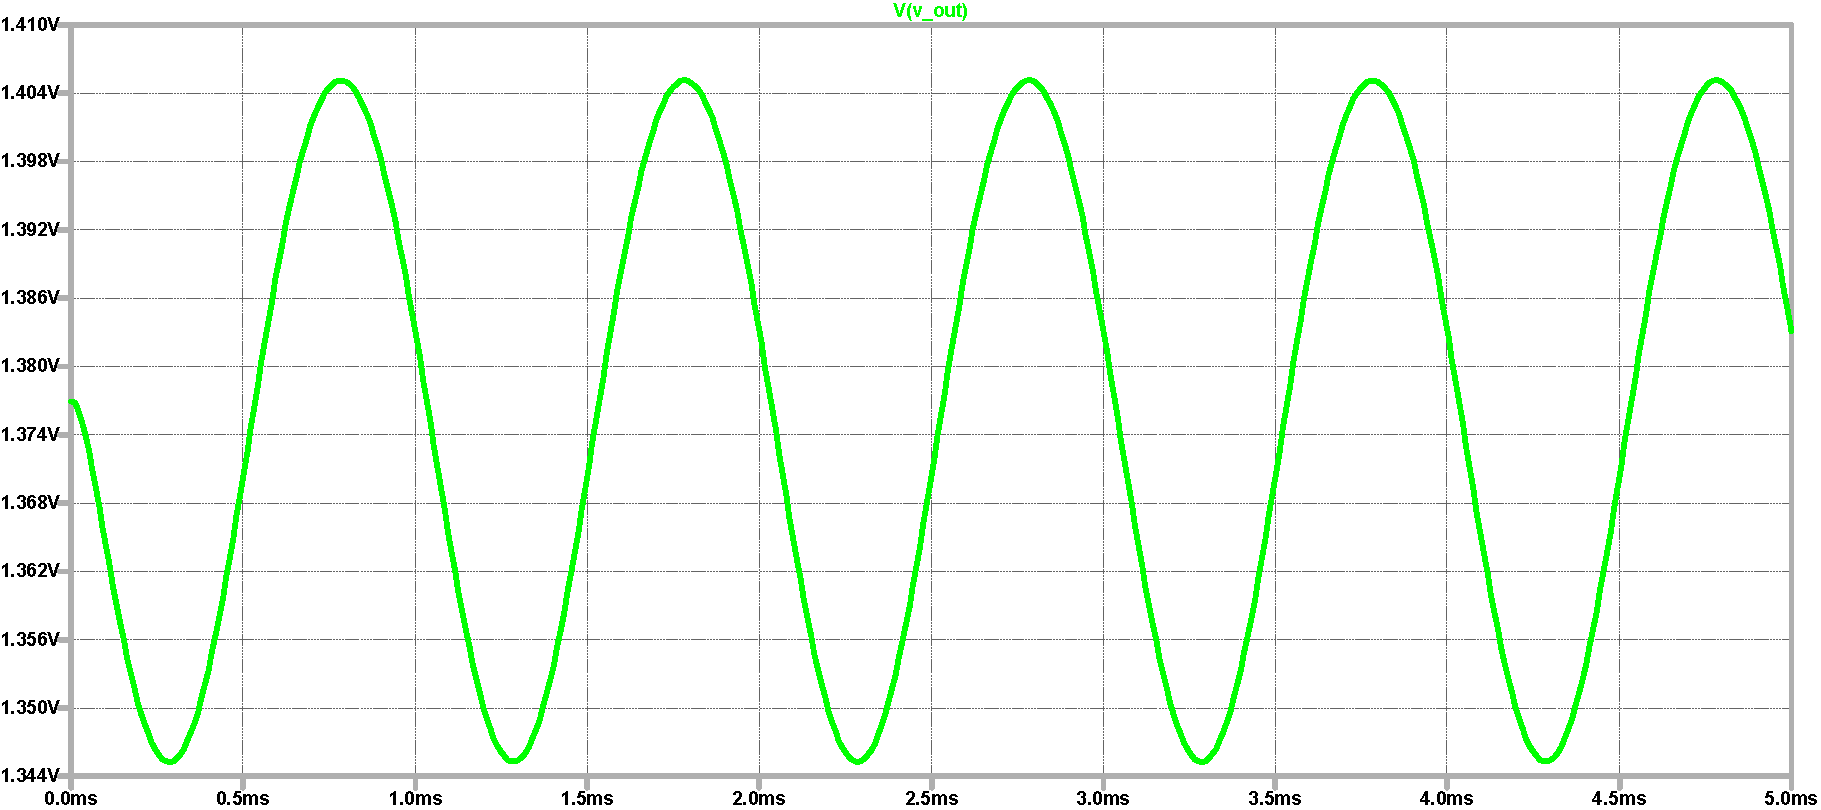
\includegraphics[width=.9\linewidth]{img/q4/transient.pdf}
\caption{\label{fig:trans-q4}Transient response}
\end{figure}

\item AC response

\begin{figure}[H]
\centering
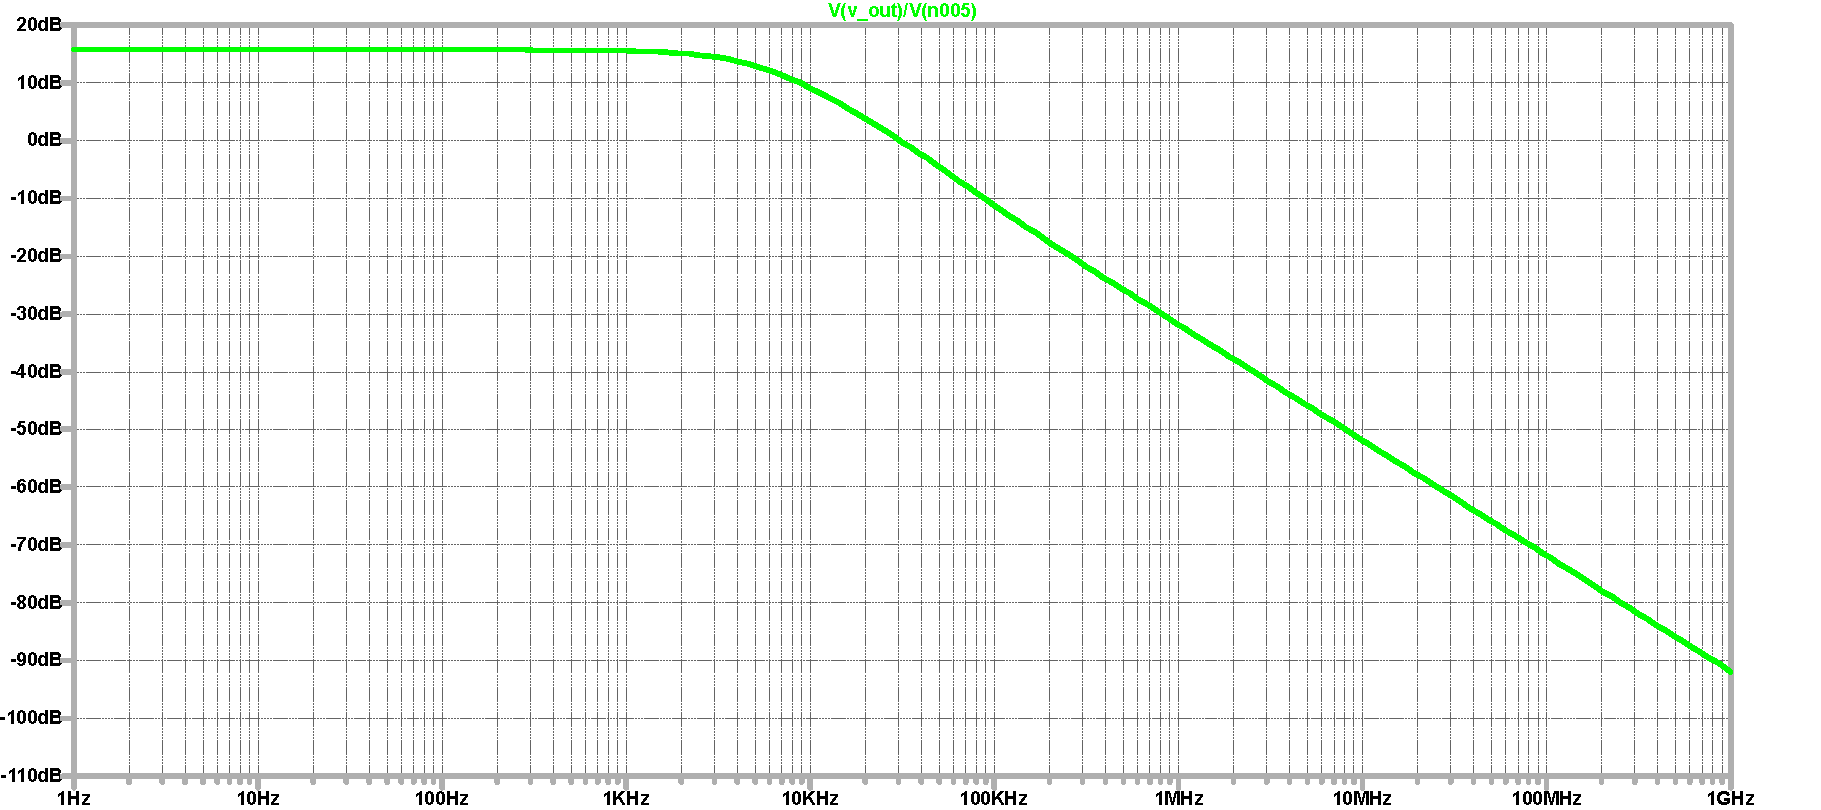
\includegraphics[width=.9\linewidth]{img/q4/gain-c.pdf}
\caption{\label{fig:gain-c-q3}Inverter AC gain}
\end{figure}

\begin{equation*}
\begin{aligned}
|\frac{V_{out}}{V_{in}}| &= 15.7 dB \\
&= 6.06 \\
\omega_{p} &= 2\pi{}f_{-3dB} \\
&= 3.35 \times 10^{4} rad s^{-1} \\
\end{aligned}
\end{equation*}

\item Gain bandwidth product, GBWP

\begin{equation*}
\begin{aligned}
|\frac{V_{out}}{V_{in}}| &= 6.06 \\
f_{-3dB} &= 5.331 kHz \\
\\
GBWP &= 32.3 kHz \\
\end{aligned}
\end{equation*}
\end{enumerate}
\end{document}
